\subsection{Methodology}
\label{se:fov}
 
\begin{figure}[p]
\begin{center}
 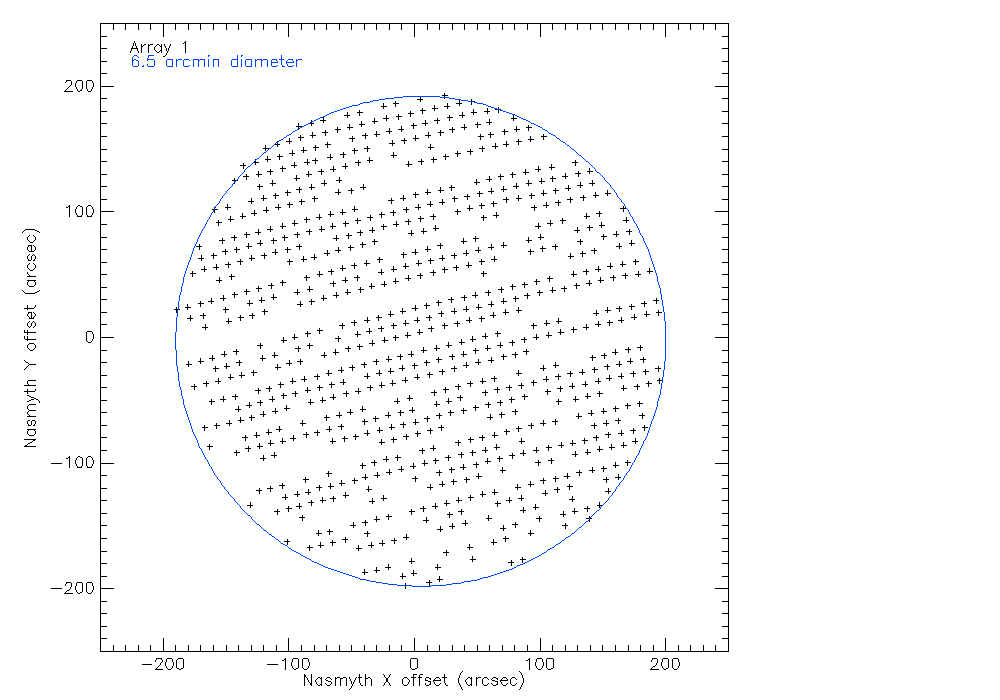
\includegraphics[angle=0, scale = 0.3]{Figures/FOV_A1.png}
 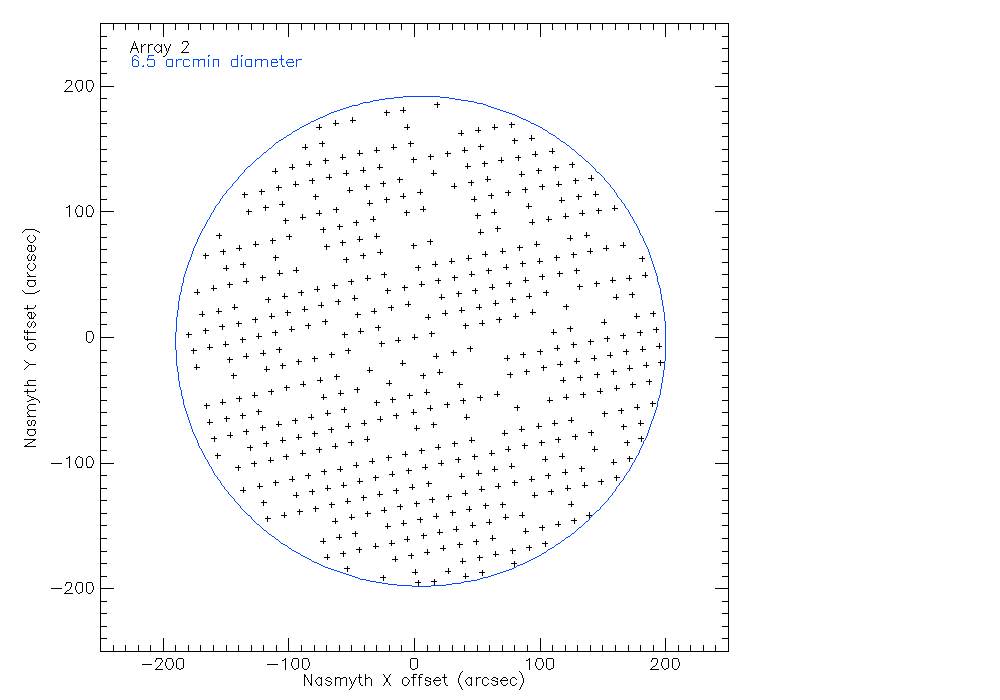
\includegraphics[angle=0, scale = 0.3]{Figures/FOV_A2.png}
 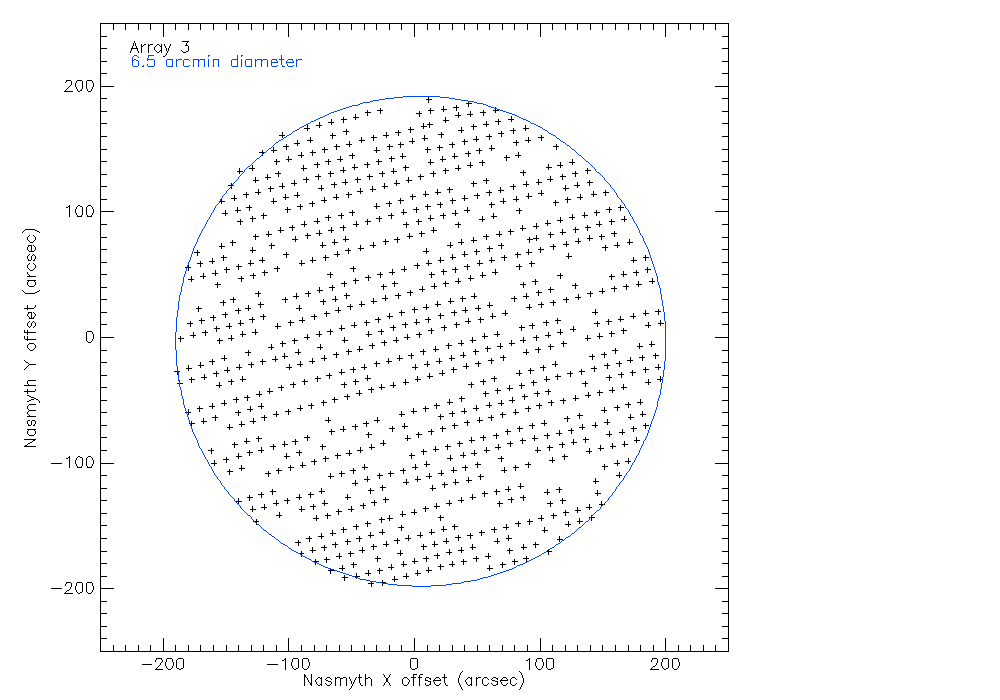
\includegraphics[angle=0, scale = 0.3]{Figures/FOV_A3.png}
\caption{Nasmyth offsets of each array, from beammap 20170226s415 on
  3C84 (N2R9).}
\label{fig:fov_ex}
\end{center}
\end{figure}

% moved to the average FOV section
%\begin{table}
%\begin{tabular}{|l|l|l|}
%\hline
%Array & Number of valid kids & Fraction of all kids\\
%\hline
%A1 & 793 & 0.75\\
%A2 & 481 & 0.83\\
%A3 & 872 & 0.83\\
%\hline
%\end{tabular}
%\end{table}

In order to determine the pointing offsets of each KID with respect to the reference sky
coordinates as commanded by the telescope tracking system, we perform a {\it beammap}, that is to say we map a bright and compact source, most of the time
a planet, with an elevation step small enough to meet Nyquist sampling at the 1-mm
beam scale, namely 4.8~arcsec. We observe this planet with a raster scan in
(az,el) coordinates, either with fixed elevation subscans or fixed azimuth
subscans. The former has the advantage of low air mass variation across a
subscan, the latter offers an orthogonal scan direction to the former: the
combination of both gives a more accurate determination of the far side
lobes. The data reduction proceeds in two steps.

\paragraph{Step 1.} We apply a median filter per
KID timeline whose width is 4~FWHM and we project one map per KID in Nasmyth
coordinates. This median filter removes efficiently most of the atmospheric and low frequency
electronic noise, albeit a slight ringing and flux loss on the
source. However, at this stage, we are only interested in the location of the
observed planet. To derive the Nasmyth coordinates from the provided (az,el)
coordinates, we build the following quantities at time~$t$ :

\begin{eqnarray}
dx_t &=& \cos el_t\, daz_t - \sin el_t\, del_t \nonumber \\
dy_t &=& \sin el_t\, daz_t + \cos el_t\, del_t \nonumber
\end{eqnarray}

\noindent {\bf FM: why not using $\delta$ as in the previous section ?}\\
\noindent {\bf FM: i don't think the $_t$ is useful}\\


where $el_t$ is the elevation of the reference pointing direction and $daz$ and
$del$ are the pointing offsets with respect to the source in azimuth and elevation as
provided by the tracking system. Note that $daz$ is already corrected by the
$\cos el_t$ factor to have orthonormal coordinates in the tangent plane of the sky
and be immune to the geodesic convergence at the poles. We then fit a 2D
elliptical gaussian on each kid map. The centroid of this gaussian is a first
estimate of the KID offsets, FWHM's, ellipticity and sensitivity. We apply a
first KID selection by removing outliers to the statistics on these
parameters. We also discard manually KIDs that show a cross-talk counter part on
their map. 
%At the end of this first step, we are ready to move to a second stage.

\paragraph{Step 2.} With the Nasmyth offsets derived in step 1, we are now able to
mask out the planet in each KID timeline. This mask is centered on the planet
location as seen by each kid, it is circular and has a radius of 60~arcsec. We
now build a template timeline (a.k.a. ``common mode'') in two steps. First, we
take the median of all samples of all KIDs that are outside this mask at a given
time $t$. This gives a first estimate of the common mode. Second, we
cross-calibrate each KID on this common mode when the KID is outside the mask
and we coadd all these KID cross-calibrated timelines when they are outside the
mask to have the final common mode. In this sum, each KID TOI is weighted by the
inverse of its variance outside the mask. Once we have this common mode in hand,
we cross-calibrate each TOI on it outside the mask and we subtract it to the
entire KID TOI. We then resume to the projection of each KID TOI in Nasmyth
coordinates like in step 1, and the 2D elliptical gaussian fit on the each kid
map. The centroid coordinates and the FWHM are now the final parameters that can
be derived on the current scan.

This analysis is repeated on all beam maps, which provides statistics and
precision on each KID parameter, together with estimates on KID performance stability.



{\bf FM : {\it precision} ? }\\
{\bf show a screen capture of Katana.}\\

% LP: j'ajoute une phrase pour referencer la Figure \ref{fig:fov}
We present an example of the FOV reconstruction in Fig.~\ref{fig:fov_ex}.

The FOV diameter is defined as 
\begin{equation}
FOV diameter = \sqrt{4 N_{tot. kids} \times gridstep^2/\pi}
\end{equation}

{\bf give the values of gridstep (pitch) both in mm and arcsec on the sky}\\

The same definition applies to ``Effective FOV'' to avoid extra multiplication
by the fraction of valid pixels

\begin{equation}
F\lambda = gridstep\times D(30m)/\lambda
\end{equation}
